\frame{
  \frametitle{Les débris spatiaux}
  \begin{minipage}{0.48\linewidth}
    \begin{itemize}
      \item Un catalogue de $15\;000$ objets de la NASA.
      \item Estimation de \textbf{$100\;000$ débris} de 1 à 10 cm dont on ne
        connait pas la trajectoire.
      \item Prolifération par collisions : pour stabiliser la
        population, enlever \textbf{5~gros débris par an}.
    \end{itemize}
  \end{minipage}
  \begin{minipage}{0.48\linewidth}
    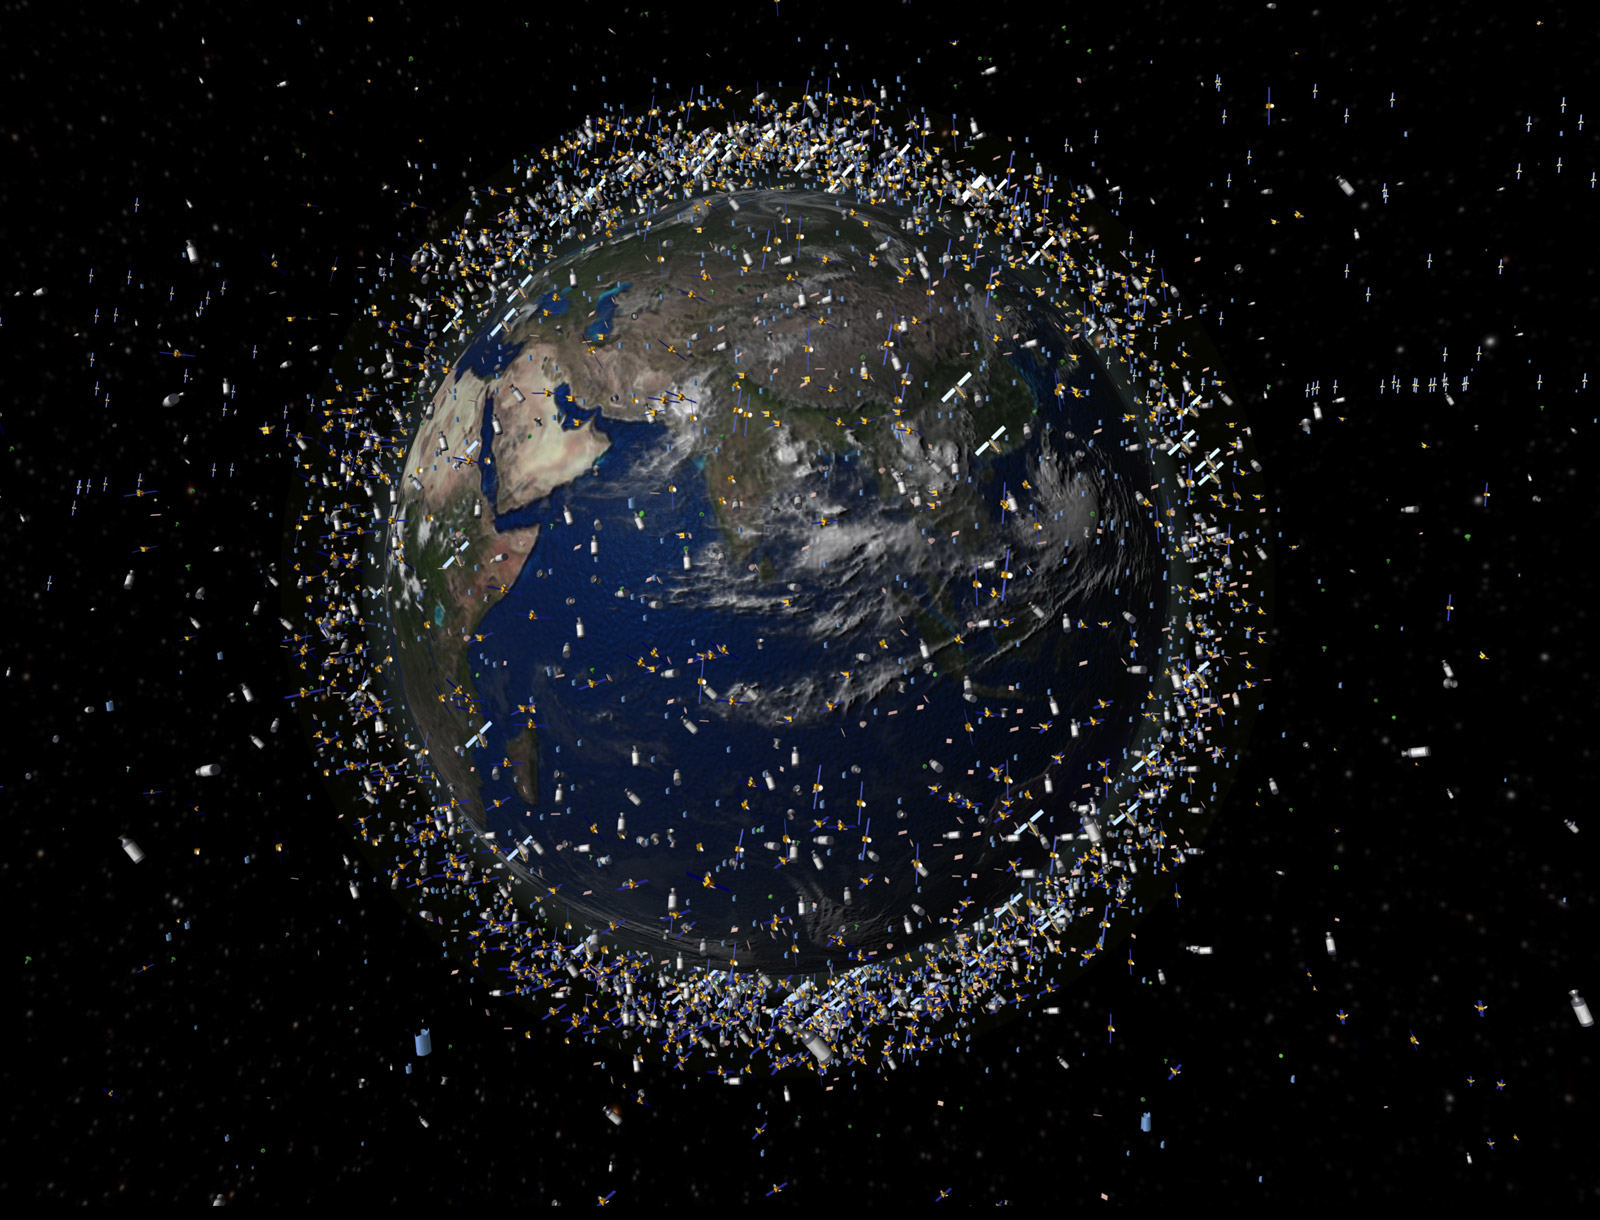
\includegraphics[width=\linewidth]{debrisSpatiaux2}
  \end{minipage}
}

\frame{
  \frametitle{Modèle}
  \begin{minipage}{0.55\linewidth}
    \begin{itemize}
    \item \textbf{Soleil}, rayon $a_{s}$, inclinaison $i_{s}$,\\
      $\triangleright$ équation du mouvement :
        \[\theta_{s}(t)=\theta_{s}(t_{0})+\omega_{s}\cdot(t-t_{0}).\]
    \item \textbf{Débris}, rayon $a_{d}$, inclinaison $i_{d}$,\\
      $\triangleright$ équation du mouvement sur l'orbite :
        \[\theta_{d}(t)=\theta_{d}(t_{0})+\omega_{d}\cdot(t-t_{0}),\]
    \end{itemize}
  \end{minipage}
  \begin{minipage}{0.43\linewidth}
    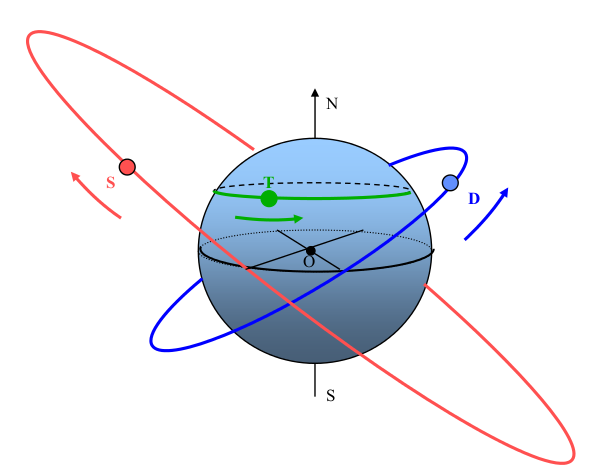
\includegraphics[width=\linewidth]{modele.png}
    \begin{itemize}
    \item \textbf{Télescope}, latitude $\varphi$, longitude
      \[\lambda_{T}(t)=\lambda_{T}(t_{0})+\omega_{T}\cdot(t-t_{0}).\]
    \end{itemize}
  \end{minipage}
}

\frame{
  \frametitle{Précession}
  \begin{minipage}{0.50\linewidth}
    \begin{itemize}
    \item \textbf{Applatissement terrestre} crée un couple autour de
      la ligne des n\oe uds.
    \item \textbf{Rotation de l'orbite} autour de l'axe $z$.\\
      $\triangleright$ précession :
      \[\theta_{o}(t)=\theta_{o}(t_{0})+\omega_{o}\cdot(t-t_{0}).\]
    \end{itemize}
  \end{minipage}
  \begin{minipage}{0.47\linewidth}
    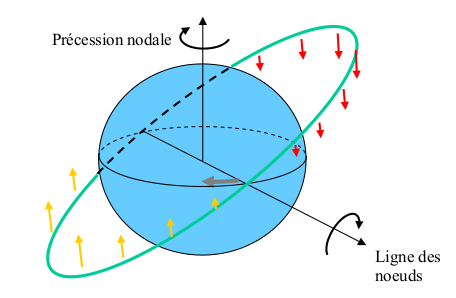
\includegraphics[width=\linewidth]{precession.png}
  \end{minipage}
}

\frame{
  \frametitle{Le problème}
  % \begin{block}
    \textbf{Problème :}
    \begin{itemize}
    \item Un téléscope observe au zénith avec un angle d'observation
      $\widetilde \alpha$. Il voit un débris quand le débris est au soleil et le
      téléscope dans la nuit.
    \item Étant donné un débris et un télescope, au bout de combien de
      temps est-on en mesure de l'observer ?
    \item Étant donné une durée d'observation, combien de télescopes
      faut-il pour observer le débris ?
    \end{itemize}
  %\end{block}
}
